\chapter{Materiais e Métodos}
\label{chap:materiais_metodos}
O metodologia empregada nos trabalhos de conclusão de curso do Centro Universitário SENAI CIMATEC é executado com base na metodologia TheoPrax que foi desenvolvida pelo instituto Fraunhofer de Tecnologia Química, situado na Alemanha. A sistemática TheoPrax tem como principal objetivo incrementar a motivação da aprendizagem através do desenvolvimento de projetos reais voltados para empresas, proporcionando a integração entre o conhecimento técnico e sua aplicação prática. Para isto, esta estrutura envolve a identificação de uma situação problema ou de uma melhoria no processo ou no produto da empresa, seu estudo e, por fim, a definição de uma proposta técnica-financeira para implementação da solução.

\section{Metodologia}
\label{sec:metodologia}
A utilização da metodologia Theoprax se restringe apenas ao gerenciamento macro do projeto e não define como a solução proposta deve ser desenvolvida. Sendo assim, o desenvolvimento do projeto, proposto no tópico \ref{sec:objetivo_geral}, será realizado utilizando o procedimento ilustrado na figura \ref{fig:metodologia_diagrama} que foi adaptado da metodologia empregada no BIR (\textit{Brazilian Insitute of Robotics}) para desenvolvimento de projetos de robótica.

\begin{figure}[H]
	\label{fig:metodologia_diagrama}
	\centering
	\caption{Metodologia empregada no desenlvolvimento do projeto solução.}
	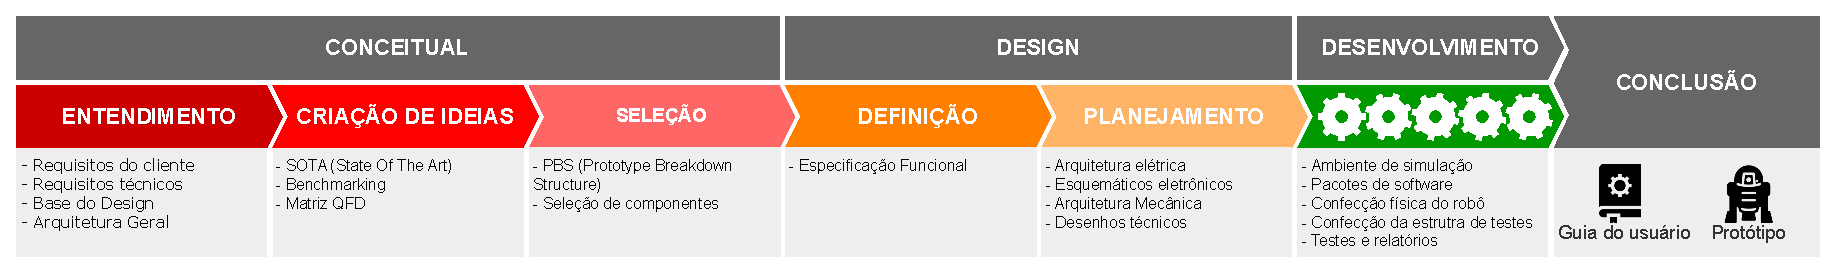
\includegraphics[width=1\textwidth]
	{Figures/metodologia_diagrama}
	\source{Própria Autoria}
\end{figure}	

Conforme Figura \ref{fig:metodologia_diagrama}, a metodologia utilizada neste projeto possui 4 etapas: Conceitual, Design, Desenvolvimento e Conclusão. Por conseguinte, cada etapa possui entradas e saídas, que vão se complementando ao longo do desenvolvimento do projeto, as quais serão explicadas nos tópicos seguintes.

\subsection{Conceitual}
\label{subsec:metodologia_conceitual}

A primeira etapa, designada como \textbf{Conceitual}, embora não explicitada no diagrama, possui como entradas as informações provenientes do cliente. Essas informações, tais como o problema proposto e os seus requisitos são utilizadas para o entendimento do projeto, servindo como ponto de partida para formulação da proposta de solução. Diante dessas informações, é possível definir os requisitos técnicos com base nos desejos do cliente (requisitos do cliente); a base do design, que consiste na definição do escopo e o que será necessário para desenvolver o projeto: meios, padrões e os principais componentes (hardware e software); e a arquiterura geral, que fornece uma visão macro de como será a interação entre o hardware e o software do robô. 

Após o entendimento do projeto, passa-se para a criação de ideias. Nesta subetapa, algumas pesquisas são realizadas para ajudar no processo de criatividade e evitar a reimplementação do que já existe no mercado. Assim, utiliza-se o SOTA (\textit{State Of The Art}), documento que aponta as principais pesquisas  e estudos sobre o tema do projeto, referenciando pesquisas acadêmicas já realizadas; e o Benchmarking, que é uma relação oriunda do mercado na qual aponta os competidores para o sistema projetado, incluindo para cada competidor critérios de avaliações importantes para o projeto. Finalizando a subetapa de criação de ideias, tem-se a Matriz QFD (\textit{Quality Functional Deployment}), em que os requisitos do cliente são confrontados com os requisitos técnicos, fornecendo à equipe de desenvolvimento do projeto os principais pontos que deverão receber maior atenção durante a elaboração do projeto. 

Por fim, após o entendimento do projeto e a formulação da ideia, parte-se para a etapa de seleção dos principais componentes do  sistema, em que primeiro elabora-se o PBS (\textit{Prototype Breakdown Structure}), uma representação do projeto com uma visão de subsistemas, apresentado através de um fluxo estruturado.

\subsection{Design}
\label{subsec:metodologia_design}
Com o conceito pré-estabelecido do sistema que será desenvolvido, parte-se para a etapa de \textbf{Design}. Nesta fase, define-se o sistema de maneira mais clara, tendo a especificação funcional como principal elemento. Este documento compreende a explicação  detalhada de cada funcionalidade do robô, contendo a definição, o objetivo, as premissas e as suas entradas e saídas. Devido ao nível de detalhes da especificação funcional, revisões em documentos anteriores, principalmente a arquitetura geral, são realizadas durante esta fase. 

No final da etapa de Design, começa-se o planejamento para o desenvolvimento técnico do projeto. Durante o planejamento é elaborado a arquitetura elétrica do robô (uma visão mais detalhada da arquitetura geral), descrevendo as formas de conexão e os protocolos de comunicação entre os elementos que compõem o sistema; os equemáticos eletrônicos, os quais são utilizados para confecção das PCIs (Placa de Circuito Impresso) que comporão o sistema; a arquitetura mecânica, apresentando os elementos mecânicos do robô; e por fim, os desenhos técnicos mecânicos, utilizados posteriormente para fabricação das peças do protótipo. 

Em conclusão, esta fase é de extrema importância, pois possibilita a geração de documentos que podem ser utilizados para a replicação do projeto. Além do mais, permite mais fluidez no desenvolvimento técnico do robô.

\subsection{Desenvolvimento}
\label{subsec:metodologia_desenvolvimento}

Após a finalização do planejamento, começa-se a etapa de \textbf{Desenvolvimento} do projeto, em que o conceito e as ideias provenientes das etapas anteriores tornam-se concretas. Nesta fase são desenvolvidos e documentados os pacotes de software, os quais englobam tanto a unidade de controle do robô quanto os \textit{drivers} dos sensores, atuadores e elementos de interação com usuário. Muito dos pacotes aqui desenvolvidos, usam a especificação funcional como guia. 

Para auxiliar no processso de desenvolvimento, um ambiente de simulação torna-se elemento vital. O ambiente de simulação permite que ideias sejam propostas e testadas sem a necessidade do uso da plataforma física, acelerando o processo de desenvolvimento num âmbito em que se possui diversas pessoas trabalhando no mesmo sistema. Não menos importante, os simuladores evitam que danos sejam causados ao robô em caso de má implementação de algum algoritmo. 

Entretanto, os ambientes de simulação não refletem completamente os aspectos físicos do mundo real. Diante disso, na fase de desenvolvimento torna-se necessário também a confecção de um ambiente real para testes. Com essa estrutura, também chamada de \textit{Mockup}, pode-se realizar testes para validar o que foi desenvolvido e produzir relatórios que podem ser entregues ao cliente  como forma de acompanhamento do desenvolvimento técnico do projeto.

\subsection{Conclusão}
\label{metodologia_conclusao}
O projeto é finalizado na etapa de \textbf{Conclusão}, em que a solução proposta é entregue ao cliente. Nesta entrega é realizado a demonstração do funcionamento do robô, utilizando um ambiente real. Também é cedido além da documentação elaborada ao longo do desenvolvimento do projeto, um documento em formato de Guia do Usuário contendo as instruções para manipulação e replicação do protótipo desenvolvido.

%--------- NEW SECTION ----------------------
\section{Descrição do sistema}
\label{sec:descricao_do_sistema}
O Doogie é um robô autônomo capaz de mapear um labirinto e descobrir qual o menor caminho do seu ponto de partida até um ponto de chegada. Sua arquitetura, ilustrada na Figura \ref{fig:arquitetura_geral}, pode ser dividida em três partes: interação com o usuário, controle do sistema e interface de hardware.
Para a interação com o usuário, o robô possuirá um Buzzer e dois \textit{Push Buttons}. Além disso, há a possibilidade de acessar o sistema do robô via SSH (\textit{Secure Shell}), por intermédio da conexão WiFi. A interface de hardware é composta por motores de corrente contínua, responsáveis pela movimentação, trabalhando em conjunto com uma ponte H e Encoders; sensores infravermelhos, dispostos na frente e dos lados, a fim de identificar paredes; e uma IMU (\textit{Inertial Measurement Unit}), responsável por fornecer a aceleração linear e a velocidade angular da plataforma móvel para complementar os dados de Odometria. O controle do sistema é embarcado dentro de uma Raspberry Pi Zero que utiliza o framework ROS para gerenciar os diversos subsistemas do micromouse.

\begin{figure}[H]
	\label{fig:arquitetura_geral}
	\centering
	\caption{Arquitetura Geral do robô Doogie.}
	\includegraphics[width=1\textwidth]
	{Figures/arquitetura_geral}
	\source{Própria Autoria}
\end{figure}

\subsection{Interface de usuário}
\label{ssec:interface_de_usuario}
O acesso à Raspberry Pi Zero é feito via SSH permitindo maior acessibilidade e segurança nos dados. O mesmo é feito remotamente através de conexão \textit{wireless}, possibilitando o acesso a linha de comandos da Raspberry bem como seu sistema de arquivos, de um outro computador.
 
O robô tem uma interface de interação com o usuário através de dois \textit{Push Buttons} e um \textit{Buzzer}. Os botões são utilizados para execução de tarefas tais como: \textcolor{red}{Listar as tarefas executadas pelos botões}. O acesso a tais dispositivos é feito através do driver do periférico GPIO (\textit{General Purpose Input/Output}) que oferece interfaces de controle utilizando as linguagens de programação Pyhton e C++.

\subsection{Interface de Hardware}
\label{ssec:interface_de_hardware}
O deslocamento do robô utiliza 2 motores de corrente contínua, acoplados à Encoders, possibilitando a obtenção de informações de posição e velocidade, com objetivo de otimizar o controle e acionamento dos motores. Além disso, para permitir que os motores girem em ambas as direções, são utilizados circuitos de ponte H.
 
Os sensores infravermelho são responsáveis por identificar obstáculos no trajeto do robô. Eles são dispostos de modo que o micromouse possa indentificar as paredes do labirinto à sua direita, esquerda e frente. Também é necessário auxílio da IMU para obtenção de dados através dos sensores acelerômetro e giroscópio para estimar a posição com maior precisão. De forma similar a interface de usuário, serão utilizados drivers para estabelecer a comunicação entre o ambiente ROS e o hardware acima descrito.

\subsection{Controle do sistema}
\label{ssec:controle_do_sistema}
A Raspberry Pi Zero é um mini computador de baixo custo e fácil acesso, capaz de reunir diversas funcionalidades em uma única placa de tamanho reduzido.  No mesmo, está instalado o sistema operacional Raspbian Buster, possibilitando a utilização do framework ROS, responsável por gerenciar os subsistemas do robô.

Os principais subsistemas desenvolvidos para o Doogie foram:
\begin{itemize}
	\item \textbf{Localização:} o labirinto pode ser modelado em uma matriz, geralmente de tamanho 16x16. Esse subsistema tem o objetivo de prover informações sobre em qual posição dessa matriz o robô se encontra (linha e coluna);
	
	\item \textbf{Percepção:} com a utilização dos sensores infravermelho, o robô pode identificar se há obstáculos ao seu redor. Esse subsistema é responsável por informar se há obstáculos na frente, direita e/ou esquerda do mesmo;
	
	\item \textbf{Planejamento:} há diversas formas de mapear e completar o labirinto. Utilizando as informações obtidas dos outros subsistemas (localização e percepção), é possível realizar o algoritmo especificado e tomar as decisões necessárias para a realização da atividade;
	
	\item \textbf{Navegação:} subsistema responsável por gerenciar as ações de navegação do robô, tais como: ir para frente, virar para direita ou esquerda, parar, dentre outros.
	
	\item \textbf{Gerenciamento de Informações:} é o subsistema responsável por receber comandos através dos botões situados no chassi do robô e fornecer o mapa do labirinto a medida em que ele é percorrido. 
\end{itemize}

%--------- NEW SECTION ----------------------
\section{Desdobramento da função qualidade}
\label{sec:qfd}
\colorbox{yellow}{Fazer uma breve descrição de como os requisitos foram levantados... e referenciar a matriz QFD em anexo}

\subsection{Requisitos técnicos e do cliente}
\label{ssec:requisitos_tecnicos_e_do_cliente}

\begin{enumerate}
	\item Documentação de fácil acesso e entendimento
		\begin{enumerate}
			\item Disponibilização de todo código desenvolvido no GitHub
			\item Disponibilização guia do usuário como Wiki no GitHub
			\item Disponibilização em um repositório no GitHub esquemáticos eletrônicos, desenhos técnicos mecânicos e seus respectivos arquivos para possível edição
		\end{enumerate}
		
	\item Uso de um sistema microprocessado comercial
		\begin{enumerate}
			\item Utilização de uma Raspberry pi como sistema microprocessado
		\end{enumerate}
		
	\item Interface intuitiva
		\begin{enumerate}
			\item Permissão ao usuário acesso remoto do terminal do sistema operacional do robô
			\item Visualização do mapa do Labirinto no RViz
			\item Disponibilização de botões e display para interação com usuário na ausência de acesso remoto
		\end{enumerate}
		
	\item Tutoriais na internet para entendimento do funcionamento do robô
		\begin{enumerate}
			\item Desenvolvimento de tutorial na ROS Wiki com os primeiros passos com robô, explicando ao usuário comandos básicos de locomoção
			\item Desenvolvimento de tutorial na ROS Wiki explicando ao usuário como implementar no robô seu próprio algoritmo de resolução de labirinto
		\end{enumerate}
		
	\item Autonomia suficiente para utilização em ao menos duas aulas consecutivas
		\begin{enumerate}
			\item Bateria recarregável 
			\item Autonomia superior a 1h40min
		\end{enumerate}
		
	\item Uso de componentes de fácil manipulação e com facilidade de aquisição
		\begin{enumerate}
			\item Uso de conectores polarizados
			\item Utilização de padrão de cores para cabos de conexão
			\item Especificação de componentes disponíveis no mercado nacional
			\item Desenvolvimento de shield de interface entre a plataforma de processamento e os sensores e atuadores
		\end{enumerate}
		
	\item Estrutura física compatível com as regras estabelecidas em competições do IEEE
		\begin{enumerate}
			\item Dimensões do robô devem ser menores que 15 x 15 x 10 cm
		\end{enumerate}
\end{enumerate}

%--------- NEW SECTION ----------------------
\section{Especificação dos componentes}
\label{sec:espc}
asjdflkdjsaf

\subsection{Estrutura analítica do protótipo}
\label{ssec:pbs}
asdkjfsdalkjf

\subsection{Lista de componentes}
\label{ssec:list}
asfkjdsahfkjs


%--------- NEW SECTION ----------------------
\section{Diagramas mecânicos}
\label{sec:diagm}
Para o design do robô, foi utilizado como um ponto de partida o TON-BOT V1.1, plataforma desenvolvida pela Ioton Technology \textcolor{red}{Colocar referência}. Além disso, uma vez que o robô a ser desenvolvido é do tipo micromouse, ele deve ter suas dimensões não superiores a uma seção retangular de 25 x 25 cm \textcolor{red}{Colocar referência}.

A partir dessas premissas e da análise feita na subseção 3.1, buscou-se um design mecânico simples e de maior leveza. Dessa forma, será utilizado como frame do robô as próprias PCIs (Placa de Circuito Impresso), buscando posicionar suas rodas de forma a mantê-las alinhadas ao centro de massa de todo o conjunto mecânico. Para tanto, uma modelagem em CAD inicialmente foi realizada através de ferramenta Solidworks, buscando iterativamente a melhor disposição de seus elementos físicos (rodas, sensores e demais componentes eletrônicos das placas).  O modelo mecânico final pode ser visualizado na \colorbox{yellow}{Figura  2}.

\colorbox{yellow}{Colocar imagens 3D do robô}

Da esquerda para direita visualiza-se as placas inferior, superior além do modelo do robô visto em perspectiva. A placa inferior possui 98 mm de comprimento e 92,90 mm de largura, enquanto a placa superior possui 75 mm de comprimento e 92,90 mm de largura. Foi necessário o uso de duas placas para melhor adequação dos componentes eletrônicos sem atrapalhar eventuais manutenções no dispositivo nem dificultar sua montagem.

%--------- NEW SECTION ----------------------
\section{Modelo esquemático de alimentação e comunicação}
\label{sec:modesq}
Com intuito de facilitar a replicação do robô por usuários que queiram utilizá-lo, optou-se pelo uso de \textit{breakout boards}, que são placas eletrônicas pré-montadas. O Doogie possui seis \textit{breakout boards}: dois conversores de tensão DC-DC, modelos MT3608 e U1V10F5, um conversor Analógico/Digital (A/D) ADS1115, uma IMU, um multiplexador analógico 74HC4051  e uma ponte H. Os demais componentes como resistores, transistores, LEDs infravermelho, fototransistores e conectores, são soldados diretamente na Placa de Circuito Impresso (PCI). Esses componentes foram distribuídos nas PCIs superior e inferior do robô, conforme \textcolor{red}{Referenciar figura}. A fim de fornecer energia elétrica para esses componentes, foi especificado uma bateria do tipo Li-Ion modelo 18650 com tensão nominal igual à 3,6 V. A arquitetura elétrica na Figura \ref{fig:arquitetura_eletrica} demonstra como tais componentes estão interligados eletricamente. A propósito de melhor visualização, o referencial de tensão (Ground - GND) foi omitido.

\begin{figure}[H]
	\label{fig:arquitetura_eletrica}
	\centering
	\caption{Representação elétrica do Doogie Mouse.}
	\includegraphics[width=1\textwidth]
	{Figures/arquitetura_eletrica}
	\source{Própria Autoria}
\end{figure}

\subsection{Diagramas elétricos}
\label{sec:diagramas_eletricos}


\subsection{Esquemas eletrônicos}
\label{ssec:esquematicos_eletronicos}
\colorbox{yellow}{Referenciar em anexo!}

%--------- NEW SECTION ----------------------
\section{Especificação das funcionalidades}
\label{sec:especificacao_das_funcionalidades}
As funcionalidades de um robô descrevem os subsistemas e a lógica de operação dos mesmos. No doogie, existem quatro funcionalidades principais: Localização, Percepção, Navegação e Usabilidade. A descrição de cada funcionalidade é mostrada nos tópicos subsequentes.

\subsection{Fluxo das informações}
\label{ssec:fluxo_das_informacoes}

\begin{figure}[H]
	\label{fig:arquitetura_eletrica}
	\centering
	\caption{Representação elétrica do Doogie Mouse.}
	\includegraphics[width=1\textwidth]
	{Figures/arquitetura_eletrica}
	\source{Própria Autoria}
\end{figure}

\subsection{Funcionalidade 1}
\label{ssec:func1}
asdfsaf

\subsection{Funcionalidade 2}
\label{ssec:func2}
asdfsaf

\subsection{Funcionalidade 3}
\label{ssec:func3}
asdfsaf

%--------- NEW SECTION ----------------------
\section{Interface do Usuário}
\label{sec:ui}
asdfadsfsdfs

%--------- NEW SECTION ----------------------
\section{Simulação do sistema}
\label{sec:sim}
asdfadsfsdfs

